\documentclass[11pt]{article}
\usepackage{amsmath}
\usepackage{stackengine}
\usepackage{graphicx}
\usepackage{caption}
\stackMath

	\addtolength{\oddsidemargin}{-.875in}
	\addtolength{\evensidemargin}{-.875in}
	\addtolength{\textwidth}{1.75in}

	\addtolength{\topmargin}{-.875in}
	\addtolength{\textheight}{1.75in}

\DeclareMathOperator{\diag}{diag}

\begin{document}
Consider a 2-D strip of material that has infinite length, but finite thickness. The strip is constrained along its bottom surface by rollers, as shown in figure \ref{fig:stripFig}.
\begin{figure}[h] 
\begin{center}
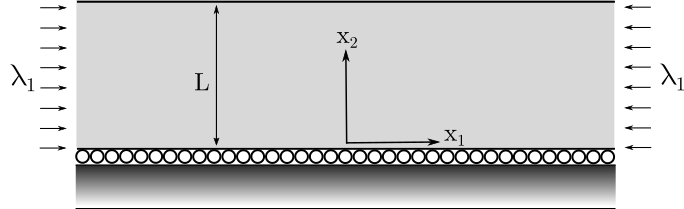
\includegraphics[scale=0.7]{compressed_strip_drawing}
\end{center}
\captionsetup{format=hang}
\caption{Diagram of the strip with finite thickness of $L$ in the $x_2$ direction, and infinite width in the $x_1$ direction. Rollers constrain the displacement in the $x_2$ direction on the bottom horizontal surface to zero. The displacement control sets the average stretch in the $x_1$ direction as $\lambda_1$}
\label{fig:stripFig}
\end{figure}

The displacement control problem will be considered. The average stretch in the $x_1$ is defined as $\lambda_1$. The loading parameter $\lambda$ will be defined as:
\begin{equation}
\lambda = 1 - \lambda_1,
\end{equation} 
where a value of $\lambda = 0$ corresponds to no displacement. The problem will be restricted to only the compressive case, where $ 0 \leq \lambda < 1 $. 

A compressible 2-D Neo-Hookean stored energy function $W$ will be used. It has the form:
\begin{equation} \label{eq:energyFunction}
W=\mu(x_2)\left[\frac{1}{2}(I_1 - 2- \ln{I_2}) + \frac{\nu}{1-\nu}(\sqrt{I_2} - 1)^2\right],
\end{equation}
where $\nu$ is a constant material parameter, and $\mu(x_2)$ is a material parameter that only varies in the $x_2$ direction. $I_1$ and $I_2$ are the principle invariants of the Cauchy-Green tensor $\mathbf{C}$ given by:
\begin{equation} \label{eq:I_functions}
I_1 = \mathrm{tr}, \mathbf{C} \qquad I_2 = \mathrm{det} \mathbf{C}.
\end{equation}
The first and second derivatives of $W(I_1,I_2)$ with the deformation gradient $\mathbf{F}$ can be found through the chain rule:
\begin{equation} \label{eq:dW_dF_chain}
\frac{\partial W}{\partial \mathbf{F}} = \frac{\partial W}{\partial I_1}\frac{\partial I_1}{\partial \mathbf{F}} + \frac{\partial W}{\partial I_2}\frac{\partial I_2}{\partial \mathbf{F}},
\end{equation}
resulting in:
\begin{equation} \label{eq:dW_dF}
\frac{\partial W}{\partial \mathbf{F}} = \mu(x_2)\left[\mathbf{F} - \mathbf{F}^{-1} + \frac{2\nu}{1-\nu}(I_2 - \sqrt{I_2})\mathbf{F}^{-T}\right],
\end{equation}
or in indicial notation:
\begin{equation} \label{eq:dW_dF_index}
\frac{\partial W}{\partial F_{ij}} = \mu(x_2)\left[F_{ij} - F^{-1}_{ij} + \frac{2\nu}{1-\nu}(I_2 - \sqrt{I_2})F^{-1}_{ji}\right].
\end{equation}
The second derivative is given by:
\begin{equation} \label{eq:d2W_dFF_pre}
\frac{\partial W}{\partial F_{ij}F_{kl}} = \frac{\partial}{\partial F_{kl}}\left\{\mu(x_2)\left[F_{ij} - F^{-1}_{ij} + \frac{2\nu}{1-\nu}(I_2 - \sqrt{I_2})F^{-1}_{ji}\right]\right\},
\end{equation}
resulting in:
\begin{equation} \label{eq:d2W_dFF}
\begin{split}
\frac{\partial W}{\partial F_{ij}F_{kl}} = \mu(x_2)\left[\delta_{ik}\delta_{jl} + F^{-1}_{jk}F^{-1}_{li} -
\frac{2\nu}{1-\nu}(I_2 - \sqrt{I_2})F^{-1}_{jk}F^{-1}_{li} \right. + \\
 \left. \frac{4\nu}{1- \nu}(I_2 - \frac{1}{2}\sqrt{I_2})F^{-1}_{lk}F^{-1}_{ji}\right].
\end{split}
\end{equation} 


Th principle solution, and later the first bifucated solution will be investigated. The total energy of the system that has no body forces or applied tractions is:
\begin{equation} \label{eq:energy}
\mathcal{E} = \int_\Omega W(\mathbf{F}) \,dA.
\end{equation}
Taking the first variation gives:
\begin{equation} \label{eq:energy,u}
\mathcal{E},_{\mathbf{u}}\cdot \delta\mathbf{u} = \int_\Omega \frac{\partial W}{\partial {F_{ij}}} \delta F_{ij} \,dA.
\end{equation}
For our principle solution, we will assume that $\stackon{\mathbf{F}}{0}$ is constant throughout the domain and is of the form $\stackon{\mathbf{F}}{0} = \diag[\lambda_1,\lambda_2]$. Then, the Priola-Kirchoff stress evaluated on this proposed solution in a orthonormal basis aligned with the $x_1$ and $x_2$ axis is:
\begin{equation} \label{eq:dW_dF_F0}
\left . \frac{\partial W}{\partial \mathbf{F}} \right|_{\stackon{\mathbf{F}}{0}} = \diag[\Pi_{11}, \Pi_{22}],
\end{equation}
where $\Pi_11$ and $\Pi_22$ are defined are:
\begin{equation*}
\begin{aligned}
\Pi_{11} &= \mu(x_2) \left [ \lambda_1 - \lambda_1^{-1} + \frac{2\nu}{1 -\nu}(\lambda_1 \lambda_2^2 - \lambda_2) \right ] , \\
\Pi_{22} &= \mu(x_2) \left [ \lambda_2 - \lambda_2^{-1} + \frac{2\nu}{1 - \nu}(\lambda_1^2 \lambda_2 - \lambda_1) \right ]. 
\end{aligned}
\end{equation*}
Enforcing the zero normal traction on the free surface at $x_2 = L$ gives:
\begin{equation} \label{eq:lambda_relation}
\Pi_{22} |_{x_2 = L} = 0  \qquad \implies \qquad \lambda_2 - \lambda_2^{-1} + \frac{2\nu}{1 - \nu}(\lambda_1^2 \lambda_2 - \lambda_1) = 0.
\end{equation}
Thus, \eqref{eq:lambda_relation} gives a relationship of $\lambda_1$ to $\lambda_2$ in the form of a quadratic. For equillibrium of this principle solution the following must be satisfied:
\begin{equation} \label{eq:eqbrm}
\mathcal{E},_{\mathbf{u}}\cdot \delta\mathbf{u} = \int_\Omega \left . \frac{\partial W}{\partial {F_{ij}}} \right |_{\stackon{\mathbf{F}}{0}} \delta F_{ij} \,dA = 0.
\end{equation}
This can be shown to be true by noting that for the displacement control in the $x_1$ direction requires that $\int_{-\infty}^{\infty} \delta F_{11} \,dx_1 = 0$. Thus, the uniform stretching meets equilibrium criteria and passes through the origin. The stability can be shown from the positive definiteness of the incremental modulii for small $\lambda_1$. (I wil type this up later) 

Now that the principle solution is determined, we will move onto the first bifurcated solution. The second variation of the energy is: 
\begin{equation} \label{eq:second_var}
(\mathcal{E},_{\mathbf{u} \mathbf{u}}\cdot \delta\mathbf{u}) \cdot \delta\hat{\mathbf{u}} = \int_\Omega  \frac{\partial W}{\partial F_{ij} F_{kl}} \delta F_{ij} \delta \hat{F}_{kl} \,dA.
\end{equation}
The first bifurcated solution $\stackon{\mathbf{u}}{1}$ occurs at a critical loading $\lambda_c$ when the following condition is met:
\begin{equation}
(\mathcal{E},_{\mathbf{u} \mathbf{u}}(\stackon{\mathbf{u}}{0}, \lambda_c) \cdot \stackon{\mathbf{u}}{1}) \cdot \delta\mathbf{u} = \int_\Omega  \left. \frac{\partial W}{\partial F_{ij} F_{kl}} \right |_{\lambda_c} \stackon{u}{1}_{i,j} \delta u_{k,l} \,dA = 0,
\end{equation}
where the variations of deformation gradient have been replaced with equivalent variations of the displacement gradient. Integrating by parts and applying divergence theorem gives:
\begin{equation} \label{eq:byparts}
\int_{\partial \Omega} L^c_{ijkl}(x_2) \: \stackon{u}{1}_{i,j} \: n_l \:  \delta u_k \: \,ds - \int_{\Omega} \left ( L^c_{ijkl}(x_2) \: \stackon{u}{1}_{i,j} \right )_{,l} \: \delta u_k \: \,dA = 0,
\end{equation}
where $\left. \frac{\partial W}{\partial F_{ij} F_{kl}} \right |_{\lambda_c}$ has been replaced by $L^c_{ijkl}(x_2)$ for brevity, and $n_{i}$ is the unit normal of $\partial \Omega$. The surface integral on the left gives the natural boundary conditions. The boundary conditions on the free surface at $x_2 = L$ are:
\begin{equation} \label{eq:bcAtL}
\left . L^c_{ij12} \: \stackon{u}{1}_{i,j} \right |_{x_2 = L} = 0, \qquad
\left . L^c_{ij22} \: \stackon{u}{1}_{i,j} \right |_{x_2 = L} = 0,
\end{equation}
which correspond to the absence of shear and normal traction, respectfully. The natural boundary condition at $x_2 = 0$ is:
\begin{equation} \label{eq:shearAt0}
\left . L^c_{ij12}(0) \: \stackon{u}{1}_{i, j}  \right |_{x_2 = 0} = 0,
\end{equation} 
which corresponds to no shear tractions at $x_2 = 0$. There is also the condition that the $x_2$ displacement at $x_2 = 0$ is fixed:
\begin{equation} \label{eq:dispAt0}
\left . u_2 \right |_{x_2 = 0} = 0 .
\end{equation}
The integrand over the domain in \eqref{eq:byparts} gives a system of two linear PDE's:
\begin{equation}
\begin{aligned}
L^c_{ij12,2} \: \stackon{u}{1}_{i,j} + L^c_{ij1l} \: \stackon{u}{1}_{i,jl} &= 0, \\
L^c_{ij22,2} \: \stackon{u}{1}_{i,j} + L^c_{ij2l} \: \stackon{u}{1}_{i,jl} &= 0 , 
\end{aligned}
\end{equation}
where the incremental moduli's exclusive dependent on $x_2$ has been used to simplify the expression. This system of PDE's can then be expanded, using the symmetry of the incremental moduli to simplify the expression, giving: 
\begin{equation} \label{eq:rawpde}
\begin{aligned}
L^c_{2112,2} \: \stackon{u}{1}_{2,1} + L^c_{1212,2} \: \stackon{u}{1}_{1,2} + L^c_{1111} \: \stackon{u}{1}_{1,11} + L^c_{1212} \: \stackon{u}{1}_{1,22}+ L^c_{2112} \: \stackon{u}{1}_{2,12}  + L^c_{1122} \: \stackon{u}{1}_{2,21} &= 0, \\
L^c_{1122,2} \: \stackon{u}{1}_{1,1} + L^c_{2222,2} \: \stackon{u}{1}_{2,2} + L^c_{2222} \: \stackon{u}{1}_{2,22}+ L^c_{1212} \: \stackon{u}{1}_{2,11}+ L^c_{2112} \: \stackon{u}{1}_{1,12}  + L^c_{2211} \: \stackon{u}{1}_{1,21} &= 0.
\end{aligned}
\end{equation}
The form of the parameter $\mu(x_2)$ will now be introduced. It will be chosen to be an exponential of the form:
\begin{equation}
\mu(x_2) = \mu_0 e^{\kappa x_2}.
\end{equation}
Then from \eqref{eq:d2W_dFF} it can be seen that all of the $L^c_{ijkl}$'s are simply constant values multiplied with $\mu(x_2)$. Then with the chosen form of $\mu$, $L^c_{ijkl,2} = \kappa L^c_{ijkl}$. Applying this to \eqref{eq:rawpde} gives:
\begin{equation} \label{eq:pde}
\begin{aligned}
\kappa L^{cc}_{2112} \: \stackon{u}{1}_{2,1} + \kappa L^{cc}_{1212} \: \stackon{u}{1}_{1,2} + L^{cc}_{1111} \: \stackon{u}{1}_{1,11} + L^{cc}_{1212} \: \stackon{u}{1}_{1,22}+ L^{cc}_{2112} \: \stackon{u}{1}_{2,12}  + L^{cc}_{1122} \: \stackon{u}{1}_{2,21} &= 0,\\
\kappa L^{cc}_{1122} \: \stackon{u}{1}_{1,1} + \kappa L^{cc}_{2222} \: \stackon{u}{1}_{2,2} + L^{cc}_{2222} \: \stackon{u}{1}_{2,22}+ L^{cc}_{1212} \: \stackon{u}{1}_{2,11}+ L^{cc}_{2112} \: \stackon{u}{1}_{1,12}  + L^{cc}_{2211} \: \stackon{u}{1}_{1,21} &= 0,
\end{aligned}
\end{equation}
where $L^{cc}_{ijkl}$ is the constant part of $L^{c}_{ijkl}$, as both equations have been divided throughout by $\mu(x_2)$.
This system of linear PDE's with constant coefficients can be separated, admitting the following form of the solution:
\begin{equation}
\mathcal{A}^2 = 
\left \{ 
\begin{aligned} 
  \stackon{u}{1}_1 &= -v_1(x_2)\sin(\omega x_1) \\
  \stackon{u}{1}_2 &=  v_2(x_2)\cos(\omega x_1)
\end{aligned} 
\right \} , \qquad
\mathcal{S}^2 = 
\left \{ 
\begin{aligned} 
  \stackon{u}{1}_1 &= v_1(x_2)\cos(\omega x_1) - v_1(0) \\
  \stackon{u}{1}_2 &=  v_2(x_2)\sin(\omega x_1)
\end{aligned} 
\right \},
\end{equation}
where $\mathcal{A}^2$ and $\mathcal{S}^2$ denote the symmetric and antisymmetric $u_1$ modes about the $x_2$ axis, respectfully. $\omega$ is an arbitrary constant that arises from the separation of the system of linear PDE's, and is realted to the wavelength of the instable mode. The $x_2$ dependence is:
\begin{equation}
v_1(x_2) = \sum_{i = 1}^{4}A_ie^{\alpha_i x_2}, \qquad v_2(x_2) = \sum_{i = 1}^{4} A_i B_i e^{\alpha_i x_2}.
\end{equation} 
These solutions can be substituted into the original system of PDE's in \eqref{eq:pde}. This results in the $\alpha_i$'s being the roots to the following quartic characteristic equation:
\begin{equation} \label{eq:characteristic}
a\alpha^4 + b\alpha^3 + c\alpha^2 + d\alpha + e = 0,
\end{equation}
where the coefficients are:
\begin{equation*}
\begin{aligned}
  a &= L^{cc}_{2222}L^{cc}_{1212}, \\
  b &= 2\kappa L^{cc}_{2222}L^{cc}_{1212}, \\
  c &= \omega^2 \left[ \left ( L^{cc}_{1122} + L^{cc}_{2112}\right )^2 - \left ( L^{cc}_{1212} \right )^2 - L^{cc}_{1111}L^{cc}_{2222} + \frac{\kappa^2}{\omega^2}L^{cc}_{2222}L^{cc}_{1212}    \right ], \\
  d &= \kappa \omega^2 \left[ \left ( L^{cc}_{1122} + L^{cc}_{2112}\right )^2 - \left ( L^{cc}_{1212} \right )^2 - L^{cc}_{1111}L^{cc}_{2222} \right ], \\
  e &= \omega^2 \left( \kappa^2 L^{cc}_{1122}L^{cc}_{2112} + \omega^2 L^{cc}_{1111}L^{cc}_{1212}. \right)   
\end{aligned}
\end{equation*}
Substituiting the form of the solution into the original system also gives the relationship for the coefficents $B_i$'s:
\begin{equation}
B_i = \frac {\omega^2 L^{cc}_{1111} - \kappa L^{cc}_{1212} \alpha_i - L^{cc}_{1212} \alpha_i^2 }
            {\omega \left (L^{cc}_{2112} + L^{cc}_{1122} \right) \alpha_i + \omega \kappa L^{cc}_{2112}}
\end{equation}
Now the solution will be substituted into the four boundary conditions. The shear traction condition at $x_2 = L$ in \eqref{eq:bcAtL}  requires:
\begin{equation}
\sum_{i = 1}^4 \left[ \omega L^{cc}_{2112} A_iB_i e^{\alpha_iL} + L^{cc}_{1212} \alpha_i A_i e^{\alpha_i L} \right ] = 0.
\end{equation}
The normal traction condition at $x_2 = L$ in \eqref{eq:bcAtL}  requires:
\begin{equation}
\sum_{i = 1}^4 \left [ L^{cc}_{2222} \alpha_i A_i B_i e^{\alpha_i L} - \omega L^{cc}_{1122} A_i e^{\alpha_i L} \right ] = 0 .
\end{equation}
The shear traction condition at $x_2 = 0$ in \eqref{eq:shearAt0} requires:
\begin{equation}
\sum_{i = 1}^4 \left [ L^{cc}_{1212} \alpha_iA_i + \omega L^{cc}_{2112} A_i B_i \right ] = 0.
\end{equation}
And lastly, the constrained vertical displacements at $x_2 = 0$ in equation \eqref{eq:dispAt0} requires:
\begin{equation}
\sum_{i=1}^4 A_i B_i = 0.
\end{equation}
These four boundary condition equations give four homogeneous equations for the four unknown $A_i$'s. These can be collected and put into matrix form:
\begin{equation}
\mathbf{M} \mathbf{A} = \mathbf{0},
\end{equation}
where $\mathbf{A}$ is the vector of amplitude $A_i$'s:
\begin{equation}
\mathbf{A} = [ A_1, A_2, A_3, A_4 ]^T.
\end{equation}
And $\mathbf{M}$ is the assembled matrix of coefficients from the boundary condition requirements. Then our first bifurcated solution occurs at the smallest $\lambda$ that satisfies:
\begin{equation} \label{eq:detM}
\mathrm{det}(\mathbf{M}) = 0.
\end{equation}
Then a procedure to find the critical load for a given wavelength mode would be to first evaluate the $\omega$ value for that mode, use that value to asseble the matrix $\mathbf{M}(\lambda)$, and then solve numerically for the lowest $\lambda > 0$ that satisfies \eqref{eq:detM}.
\end{document}





